%! TEX root = ../../main.tex

\subsection{Non-Technical Metaphor}%
\begin{wrapfigure}{r}{5cm}
  \begin{center}
    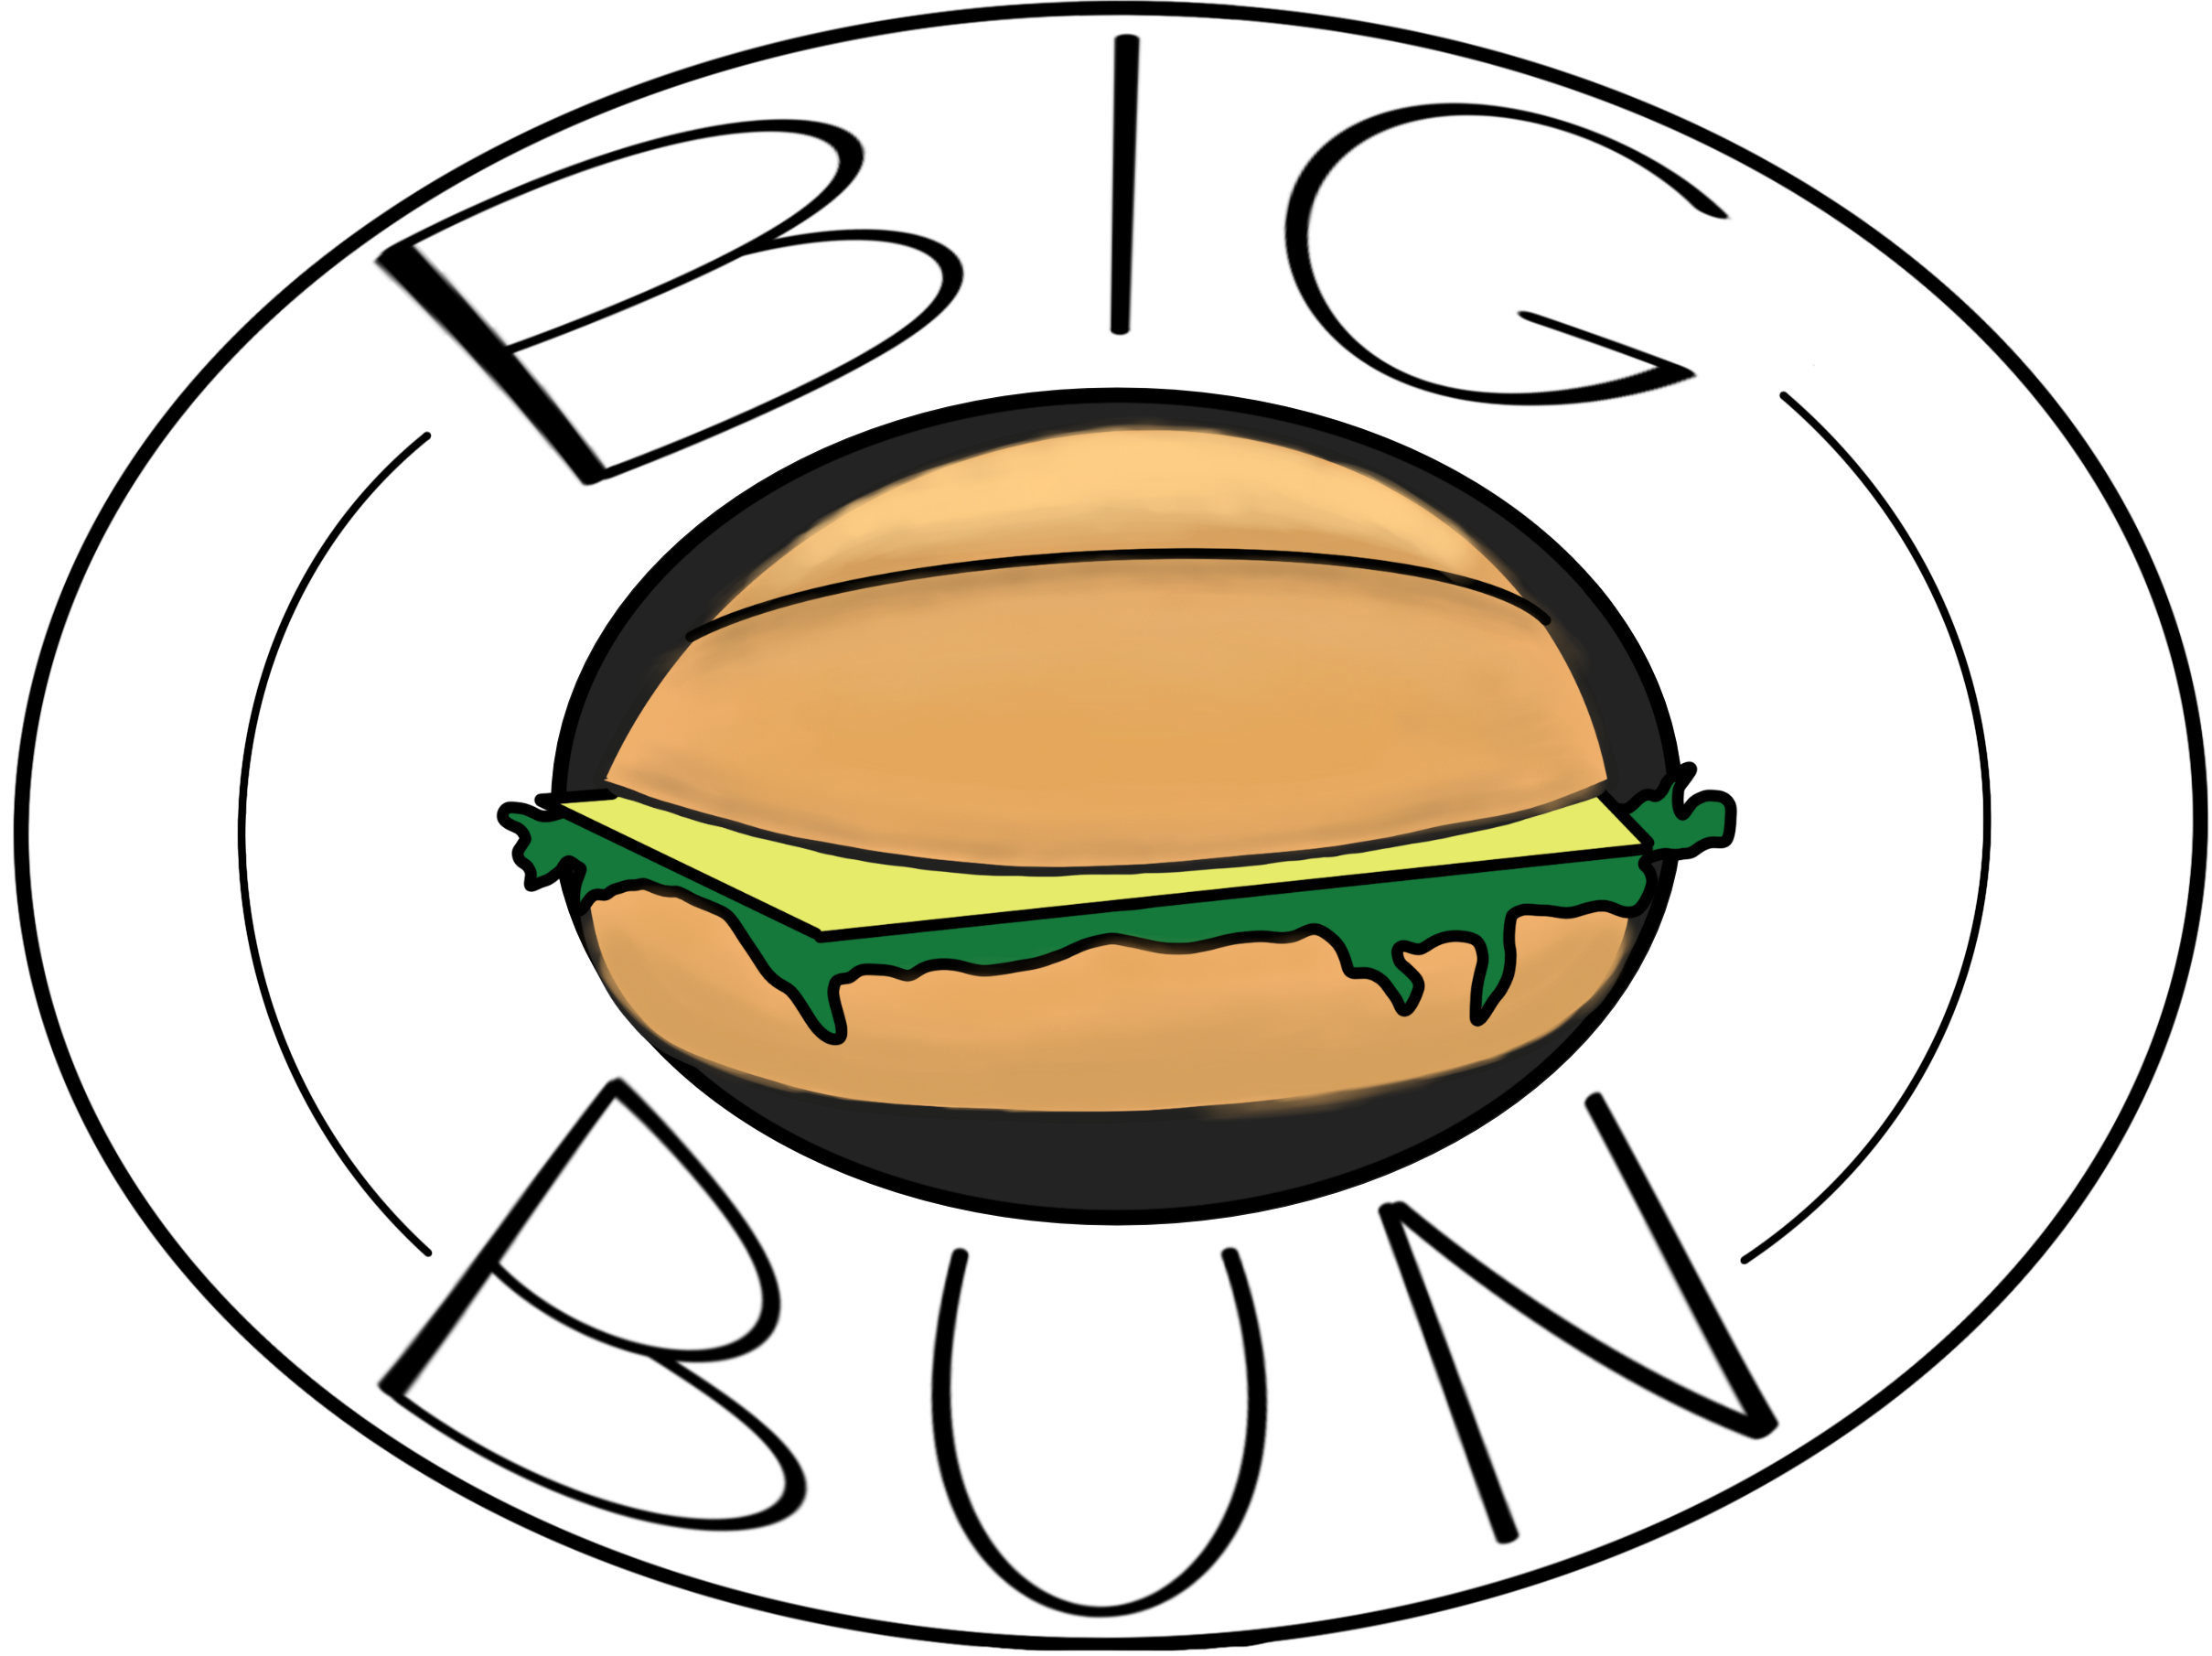
\includegraphics[width=4cm]{images/figures/big_bun_logo.png}
  \end{center}
  \caption{Imaginary \textit{BigBun} bakery logo
  \autocite{WiesemannImaginaryBigBunbakery2019}.}%
  \label{fig:big_bun_logo}
\end{wrapfigure}
It is three in the morning at the regional \textit{BigBun} bakery. Though the
population is still asleep, the work is already taking its course here.
BigBun supplies a large part of the region with freshly baked goods every
morning. Thousands of residents in the region enjoy the rolls that are produced
in this factory every day. At BigBun however, not only bread and rolls are
being made. Every day, cakes muffins and other sweet pastries leave the factory
to be consumed by the local residents.

The key to the bakery's success is its uncommon means of production. Instead of
one team that prepares one item, e.g.\ a chocolate cake, the production is
split into many small parts. First, multiple small teams prepare the doughs.
Due to the factory's high variety of baked goods, a set of base doughs
consisting of sponge, sourdough, puff pastry and yeast dough are consistently
being produced. Next to the in-house dough production, BigBun also produces its
own fillings and toppings for cakes and prepares the ingredients that go into
the making of their breads and rolls. Depending on the item that is then formed
using one of these doughs, the necessary parts are put together. In order to
e.g.\ make a chocolate muffin, a chocolate filling is added to the sponge base
dough. After baking, an additional chocolate topping is added to make the
muffin even more chocolaty.

Even though so many customers get their baked goods from BigBun's factory, the
packaging floor in the bakery is relatively empty. After the employees finish a
product, it is continuously packaged and labelled with the production date.
Next, the packaged products are shipped to the local baking shops without any
further interventions by the employees working on the production floor. Once
the trucks are loaded, the drivers are instructed to ship the baked goods off
as fast as possible; only then the freshest quality can be guaranteed.

At eight in the morning, Maria gets on her bike. It is Friday and she only has
to be late in at work. After a short ride, she reaches her local baking shop,
gets off her bike and buys two rolls. They taste as good as always even if she
never knew what went into making them; or maybe that is why they taste so
great.

\rule{2cm}{0.4pt}

Even though a healthy breakfast surely contributes to the field of computer
science, this thesis examines the workings of microservices that are being
continuously deployed. In the story above, every baking product represents a
microservice architecture. The parts, e.g.\ a topping and filling, that go into
the making of a product, e.g.\ a cake, can be interpreted as individual
microservices. The packaging of products can be directly translated to the
packaging of microservices into Docker images. The speed at which the baked
goods are delivered to shops in the area can also be compared to the speedy
continuous delivery of microservices that this thesis strives to explore.
Lastly, the goal is that the production and delivery processes are entirely
transparent for the consumer; regardless of whether the consumer eats baked
goods or uses virtual services.
